\documentclass[conference, a4paper,10pt,twocolumn]{IEEEtran}

\usepackage{graphics} % for pdf, bitmapped graphics files
\usepackage{epsfig} % for postscript graphics files
\usepackage{mathptmx} % assumes new font selection scheme installed
\usepackage{times} % assumes new font selection scheme installed
\usepackage{amsmath} % assumes amsmath package installed
\usepackage{amssymb}  % assumes amsmath package installed
\usepackage{psfrag}
\usepackage{subfigure}
\usepackage{cite}
\usepackage{amsthm}
\usepackage{flushend}

% correct bad hyphenation here
\hyphenation{op-tical net-works semi-conduc-tor IEEEtran}

\begin{document}

\title{A simple approach to WSN monitoring}

% avoiding spaces at the end of the author lines is not a problem with
% conference papers because we don't use \thanks or \IEEEmembership

% use only for invited papers
%\specialpapernotice{(Invited Paper) }

% make the title area
\maketitle
%\footnote{}
\begin{abstract}

We propose and explore the use of a very simple concept including data encoding
that can be used to enable urgent applications for Wireless Sensor Networks (WSN), 
for a wide range monitoring tasks and data collection. We also show how data can 
be distributed, shared stored and plotted on different platforms. The overall 
concept follows a straight forward unix-style format. Data is in ASCII and labeled 
with simple tags. 
It's designed to be easy to debug with low complexity and protocol support. We found 
this an alternative for monitoring applications and are using the format and ecosystem 
in long term field tests and projects.


\end{abstract}

\begin{IEEEkeywords} 
Internet of Things, IoT, 6LowPAN, Wireless sensor networks, WSN, Contiki, RIME
 \end{IEEEkeywords}


% no keywords

% For peer review papers, you can put extra information on the cover
% page as needed:
% \begin{center} \bfseries EDICS Category: 3-BBND \end{center}
%
% for peerreview papers, inserts a page break and creates the second title.
% Will be ignored for other modes.
% \IEEEpeerreviewmaketitle

\section{Introduction}
\label{sec:intro}
 

The motivation for this work is the need for innovative solutions to use the advances 
WSN and IoT research. While some areas is still under development the need for the
working solutions to address urgent applications was discovered. Also there were 
strong needs for simple installation, including setup, minimal configuration and 
effective debugging.

Microcontrollers are available, even microcontrollers with builtin radio transceivers 
as AtMega128RFA1 ~\cite{ATMEGA}. Implementing a IEEE 802.15.4 ~\cite{802154} also operating 
systems like Contiki is available ~\cite{CONTIKI} and mature. Contiki includes RIME ~\cite{CONTIKI} 
which is a very small and simple protocol for WSN communication.


In section ~\ref{sec:needs} , we discuss a more detailed needs and requirement analysis for the use cases
In section ~\ref{sec:implementation}, we present details about current implementation  
In section ~\ref{sec:experince}, we present an installation and actual usage
Finally, in section ~\ref{sec:conclusion}, we present our conclusions and suggestions for further studies.
 
\section{Needs and requirements}
%%\label{sec:Needs and requirements}
\label{sec:needs}


Different projects has motivated us for this work. One of the recent use cases is wireless sensor 
networks for monitoring and environmental monitoring.
Such networks are often deployed in remote areas with little or no power supply~\cite{UBIQUI}.  
Our low power hardware can be placed in deep sleep between measurements and transmissions.  The key 
components in our design include  Contiki-OS~\cite{CONTIKI} running on Atmel ATMega128RF~\cite{ATMEGA} 
integrating an MCU, an IEEE 802.15.4-compatible~\cite{802154} radio transceiver and an 8-channel 10-bit 
AD-converter. This component has been used to design a WSN mote with some additional components such 
as an EUI64 address chip, voltage converters, a temperature sensor, etc. When in deep sleep, the MCU 
itself consumes ~1$\mu$A and the entire mote ~10-15$\mu$A. When transmitting, the mote consumes 
~20mA. At 3V, this means ~60mW. 

The performance and coverage of the IEEE 802.15.4 depending on a lot of factors. Antenna, output
power and of course transmission disturbances but with PCB-antenna 100m line of sight and beyond 
is possible. This can have negative impacts in high density networks but for simple and small and
medium scale installations this can an advantage.


\section{Implementation}
\label{sec:implementation}


\subsection{Network topology}

IoT devices and sensors has three major mapping to the Internet. The 
or node cen exposed via

\begin{itemize}

\item Native IP address. Ether IPv4 or IPv6. 6LowPAN constitutes IPv6


\item Via a IP gateway. Gateway can of course have IPv4 or IPv6. Protocol
can be any native IP protocols or IP protocols specially designed 
for constrained applications like CoAP or MQTT etc. The gateway 
translates between two standardized internet protocol stacks. 


\item  Via IP gateway but in this case a non IP address are used on
the nodes examles Contki's RIME, Zigbee . The gateway translates 
between two protocol stacks. 

\end{itemize}

I our implementations we're using RIME on the WSN-nodes. I should
be pointed out that our TDF data tagging does not require this.

RIME is a lightweight protocol with a very low overhead. Header is 
16 bit's. The current implementation uses a RIME broadcast network
the 16 bit source address is composed by the unique EUI64 address
chip on each node this to get an unique RIME-address. 

\subsection{Report and sink nodes}

A report or broadcast node report the sensor data from local 
node, temp, RH or any more other connected instruments or 
sensors.

This report is done periodically. The radio is only active
during the sending the report which is a very short time.
Figure ~\ref{fig:bcast} illustrates this.

As a result the whole Micro Controller Unit (MCU) be in deep 
sleep and be woken up by a timer and to send it's data.

The sink node or receiving node is listening and collecting
the broadcast reports. This node is connected to the IP gateway
using USB over the TTL-UART.  There can be several sink nodes
in a network. This sink node can itself have sensors and to
report the gateway.

\subsection{Power needs}

As the network is unsynchronized the sink node must be listing
all time. This gives a higher current consumption on the sink node. 
In our case about 18mA. The new version of the AtMega128RF chip 
claims to have reduced consumption in listening mode. ~\cite{ATMEGA}

While the sink node needs some power all reporting nodes 
can spend almost it's time inte deepest sleep. Just to woken 
up by a timer read the disired sensors and go to the deepest 
sleep again. 

The memory oscilloscope traces in figure~\ref{fig:bcast} 
and figure~\ref{fig:bcast-detail} show the current consumption 
of the MCU when the radio transmits one Contiki RIME~\cite{RIME} 
broadcast packet per second. 
We see short spikes at 17mA. In this experiment, the MCU sleep 
mode was changed from ``Idle'' to ``Power save'' after four seconds.

The authors has worked on a new and innovative power design 
for sensor nodes. The design is based on the novel advances 
in supercapacitor technology. In the mentioned work ~\cite{LICCAP}  
a reporting has shown to run 6 weeks reporting every minute
on a single Lithium-Ion-Capacitor. The time to fully charge 
a capacitor is in minutes and can be done by a solar panel.

\begin{figure}
\centering
    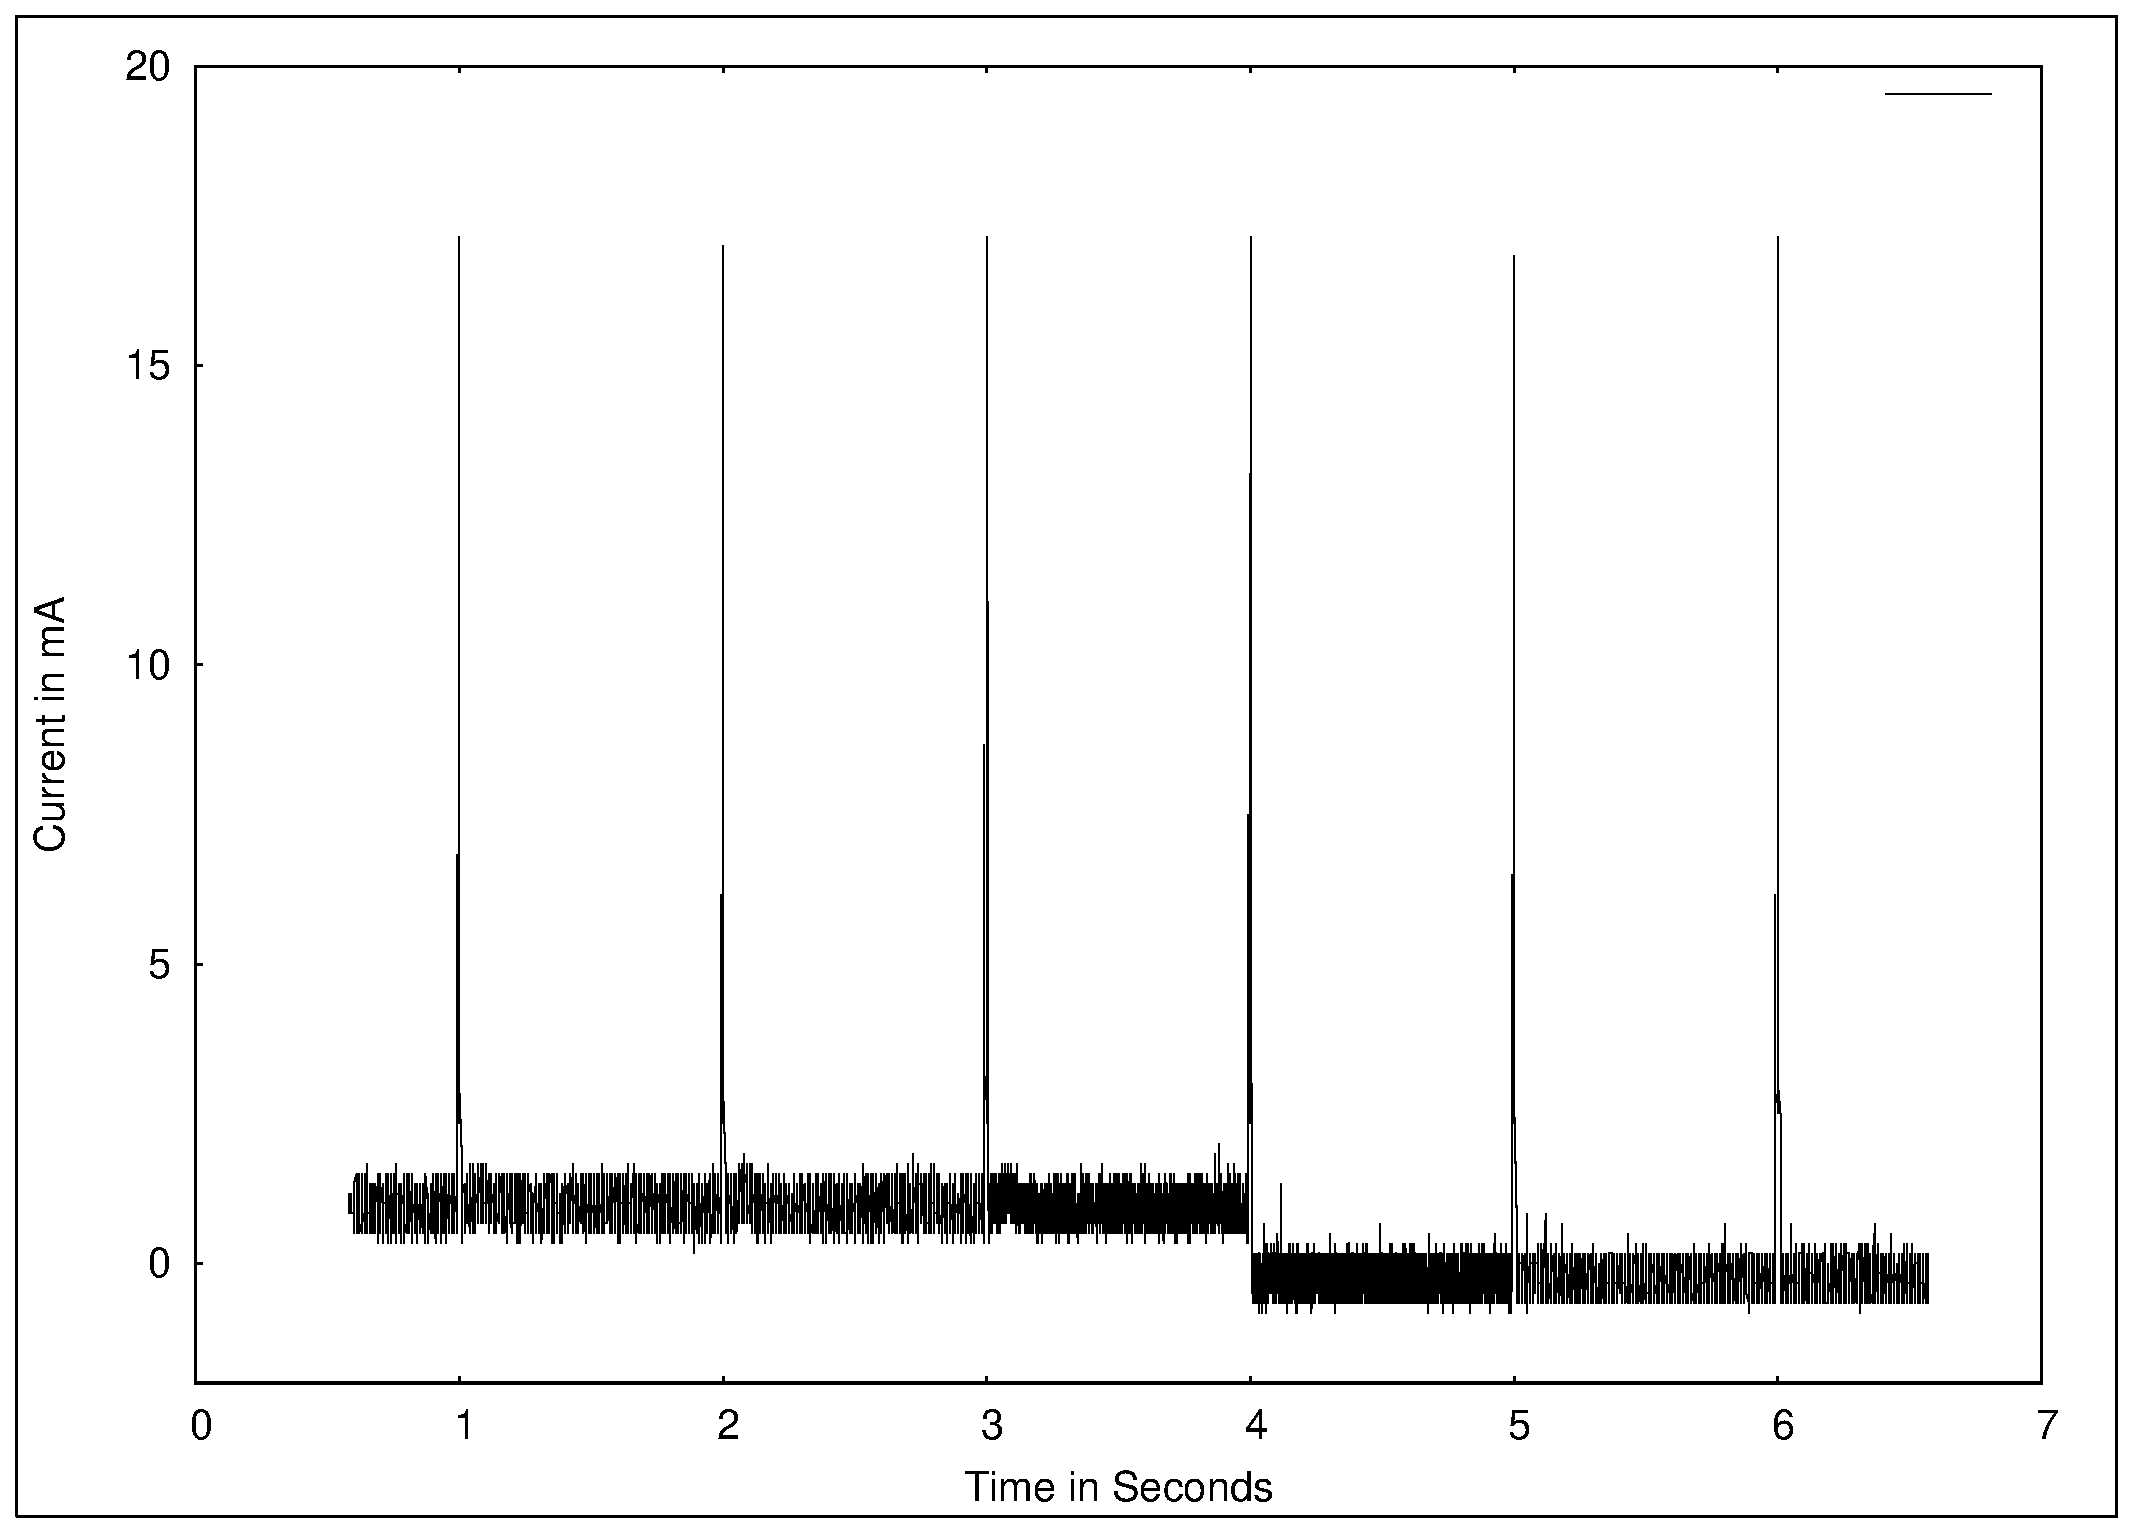
\includegraphics[width=3.4in]{bcast.eps}
    \caption{Periodic broadcast of Contiki RIME packets with 1 sec interval with ATMega128rfa1 ieee 802.15.4 radio output at 3dBm using MCU Sleep mode “IDLE” during the first 4 seconds and MCU sleep mode “PWR-SAVE” thereafter.}
    \label{fig:bcast}
\end{figure}


\begin{figure}
\centering
    \includegraphics[width=3.4in]{bcast-detail.eps}
    \caption{Close-up of one of the transmissions with MCU in Sleep mode in PWR-SAVE}
    \label{fig:bcast-detail}
\end{figure}



\subsection{Data format}
Here
Stateless vs stateful monitoring can be discussed. 


\subsection{Gateway}
The gateway gives IP connectivity to the WSN network  in other words 
all sensor sensor nodes. In our case we're using TCP for commnuction 
with the gateway.  sensd ~\cite{sensd} is the used a gateway implemeted
as a unix style daemon. Typically sensd has a sink node connected over 
USB. Sensd reads all data report from the sink node. 

When a TCP client is connected to sensd all reports received are 
distributed the client using TCP. There can be may TCP clients 
connected to the gateway at the same. All shaing the same data.
Send acts like a hub or rendez-vous point for the WSN  network.

As data is encoded in ASCII simple TCP utilities like nc, netcat, 
telnet or web browsers can be used to monitor the data. Also there 
are specialized apps for telephones. 

\subsection{Gateway and proxy}



\subsection{Plot and utilities}
Here

\subsection{App support}
Here we discuss Read Sensors App  ~\cite{read-sensors}

\subsection{Data repository and storage}
Here

\section{Experiences and Installations}
\label{sec:experince}

\section{Conclusions and further work}
\label{sec:conclusion}

We see research directions to follow:

\begin{itemize}
\item Access control of nodes and data. 

\item Merge of data flows 

\item If possible an more compact data representation and alinment to CoAP, MQTT etc

\end{itemize}

Issues for further study include: 

\begin{itemize}
\item Scalability 
\item How size of WSN network.

\item Security
\item How data integrity and security

\end{itemize} 

The authors are currently involved in field studies including these issues

\begin{thebibliography}{1}

\bibitem{UBIQUI} Amos Nungu, Robert Olsson, Bj\"{o}rn Pehrson. \emph{Implementation of Inclusive Ubiquitous Access}. 
Journal of Wireless Personal Communication, 2012

\bibitem{6LOWPAN}  Z. Shelby and C. Bormann, \emph{6LoWPAN: The Wireless Embedded Internet}
Wiley, Ed.Wiley, November 2009

\bibitem{802154}  \emph{IEEE 802.15.4}. 
[Online]. Available: http://www.ieee802.org/15/pub/TG4.html. [Accessed: 21-February-2012]

\bibitem{CONTIKI}  \emph{The Contiki Os.}. 
[Online]. Available: http://www.contiki-os.org/. [Accessed: 29-February-2012].

\bibitem{RIME} Adam Dunkels. \emph{Rime - a lightweight layered communication stack for sensor networks}.   In Proceedings of the European Conference on Wireless Sensor Networks (EWSN), Poster/Demo session, Delft, The Netherlands, January 2007.

\bibitem{ATMEGA} Atmel Corporation. \emph{ATmega128RFA1}. 
[Online]. Available: http://www.atmel.com/devices/ATMEGA128RFA1.aspx. [Accessed: 21-February-2012].

\bibitem{ATMEGAR2} Atmel Corporation. \emph{ATmega128RFR2}. 
[Online]. Available: http://www.atmel.com/devices/atmega128rfr2.aspx?tab=documents [Accessed: 01-July-2015].


\bibitem{RSS2} Radio Sensors mote. \emph{RSS2}. 
[Online]. Available: http://radio-sensors.com/ [Accessed: 16-June-2015]

\bibitem{LICCAP} Robert Olsson, Bj\"{o}rn Pehrson. \emph{Powering devices using ultra-capacitor batteries}
[Publishing Pending]

\bibitem{UBIQUISTATUS} [Amos Nungu, Robert Olsson, Bj\"{o}rn Pehrson, Jiawei Kang, Daniel Kifetew, Alisher Rustamov]. \emph{Inclusive Ubiquitous Access - A Status Report}. 
Africom, Younde, Nov 2012

\bibitem{SBN} SBN. \emph{IL2213 WSN-Projects Fall 2011.}. 
[Online]. Available: http://www.tslab.ssvl.kth.se/csd/files/wsn/index.html. [Accessed: 21-February-2012].

\bibitem{sensd}  \emph{sensd gateway}. 
[Online]. Available: https://github.com/herjulf/sensd [Accessed: 16-June-2015]

\bibitem{read-sensors}  \emph{Read-Sensors Android app}. 
[Online]. Available: https://github.com/herjulf/Read-Sensors [Accessed: 16-June-2015]


\bibitem{ODROID} \emph{Odroid U3 and C1}
[Online]. Available: http://www.hardkernel.com [Accessed 5-April-2015]
\end{thebibliography}
\end{document}

